\documentclass[a4paper]{article}
\usepackage[UTF8]{ctex}
\usepackage[a4paper,margin=1in]{geometry}
\usepackage{graphicx}
\usepackage{float}
\usepackage{listings}
\usepackage{booktabs}
\usepackage{hyperref}
\usepackage{fancyhdr}
\usepackage{lastpage}
\usepackage{color}
\usepackage{xcolor}
\usepackage{indentfirst}        % 首段缩进
\setlength{\parindent}{2em}     % 缩进2字符
\usepackage{zhnumber}           % 中文编号
\usepackage[dvipsnames]{xcolor}
\usepackage{amsmath}

% ===== 个人信息与实验信息配置 =====
\newcommand{\projname}{PersonalTax}
\newcommand{\reporttitle}{面向对象程序设计文档}
\newcommand{\stuno}{23336179}
\newcommand{\authorname}{马福泉}
\newcommand{\major}{计算机科学与技术}
\newcommand{\adviser}{李文军}
\newcommand{\startdate}{2026年3月}
\newcommand{\labenddate}{2026年3月}
\newcommand{\labroom}{B201}

% ===== 页眉页脚设置 =====
\pagestyle{fancy} 
\fancyhf{}      
\fancyhead[L]{\kaishu \projname}      
\fancyhead[C]{\kaishu \reporttitle}    
\fancyhead[R]{\kaishu \authorname} 
\fancyfoot[C]{第 \thepage 页，共 \pageref{LastPage} 页} 
\renewcommand{\headrulewidth}{0.4pt}
\renewcommand{\footrulewidth}{0pt}

% ===== 代码高亮配置 (适应 Java) =====
\definecolor{NavyBlue}{RGB}{0,0,128}
\lstset{
    language=Java,
    basicstyle=\ttfamily\small,
    commentstyle=\color{gray}\itshape,
    keywordstyle=\color{blue}\bfseries,
    stringstyle=\color{red},
    breaklines=true,
    frame=single,
    numbers=left,
    numberstyle=\tiny\color{gray},
    tabsize=4,
    showstringspaces=false,
    captionpos=b,
    escapeinside={\%}{\%}
}

\begin{document}

% ==================== 封面 ====================
\begin{titlepage}
    \centering
    
    % 若没有校徽图片，可将下面这行注释掉
    
\includegraphics[width=10cm]{img/SYSULogo.png}

    \vspace{1em}
    {\Large \kaishu \projname \par}
    \vspace{3em}

    {\fontsize{36pt}{40pt}\kaishu \selectfont \boldmath \reporttitle\par}
    \vspace{2em}
    \vspace*{\fill}

    \begin{center}
    {\Large
    \makebox[5em][s]{学号}:\underline{\makebox[15em][c]{\kaishu \stuno}}\\[1em]
    \makebox[5em][s]{姓名}:\underline{\makebox[15em][c]{\kaishu \authorname}}\\[1em]
    \makebox[5em][s]{专业}:\underline{\makebox[15em][c]{\kaishu \major}}\\[1em]
    \makebox[5em][s]{指导教师}:\underline{\makebox[15em][c]{\kaishu \adviser}}\\[1em]
    \makebox[5em][s]{起始日期}:\underline{\makebox[15em][c]{\kaishu \startdate}}\\[1em]
    \makebox[5em][s]{结束日期}:\underline{\makebox[15em][c]{\kaishu \labenddate}}\\[1em]
    \makebox[5em][s]{实验地点}:\underline{\makebox[15em][c]{\kaishu \labroom}}
    }
    \end{center}

    \vspace*{\fill}
\end{titlepage}

% ==================== 目录 ====================
\tableofcontents
\newpage

% ==================== 正文 ====================

\section{需求分析与对问题的理解}

本实验的核心目标是设计一个基于命令行的个人所得税计算系统。根据我国税法规定，应缴纳的个人所得税依赖于“应纳税所得额”（即总收入减去免征基数/起征点），并按照超额累进税率表进行分段计算。

我认为本系统在设计时面临的核心痛点在于\textbf{政策的易变性}：
\begin{enumerate}
    \item \textbf{起征点变化}：根据课程文档，历史上的起征点曾经历过 800元、1600元、3500元乃至 5000元的多次调整。
    \item \textbf{税率分级变化}：税率的级数和对应的百分比也可能随立法修订而改变（例如从 9级 调整为 7级）。
\end{enumerate}
因此，如果采用传统的结构化程序设计，将所有的税率区间和百分比通过冗长的 \texttt{if-else} 语句硬编码（Hardcode）在函数内部，未来一旦政策变动，代码的修改成本将极高，且极易引入错误。

本系统遵循\textbf{面向对象设计原则}，实现数据与逻辑的解耦，以保证程序具备良好的\textbf{可复用性}与\textbf{可扩展性}。

\section{面向对象建模与架构设计}

\subsection{实验结构说明}
本实验的项目目录结构进行了明确的模块化划分，将源代码、说明文档、自动化脚本与测试用例进行了解耦。具体的物理目录结构如下：
\begin{verbatim}
学号姓名/ (根文件夹)
│
├── src/                # 存放所有 .java 源代码文件
│   ├── TaxApp.java
│   ├── TaxCalculator.java
│   └── TaxRateItem.java
│
├── doc/                # 存放 javadoc 生成的 HTML 说明文档 (index.html 等)
│
├── scripts/            # 存放编译与运行脚本
│   ├── build.bat       # 编译脚本
│   ├── run.bat         # 运行脚本
│   └── regression.bat  # 回归测试脚本 (如有)
│
├── test_cases/         # 存放测试用例相关文件 (输入数据、预期结果等)
│
├── design.pdf          # 面向对象设计文档 (包含 UML 类图等)
└── readme.txt          # 个人信息及实验体会
\end{verbatim}

\subsection{架构图设计}
在宏观上采用了清晰的三层架构设计，系统包图与组件之间的单向依赖关系如图 \ref{fig:architecture} 所示。
\begin{figure}[H]
    \centering
    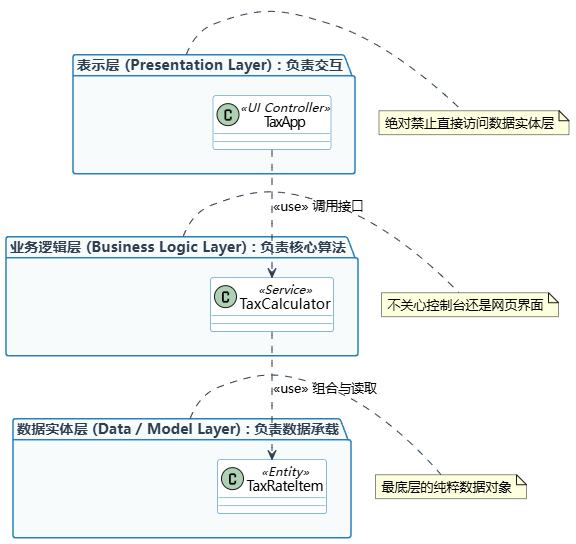
\includegraphics[width=0.75\textwidth]{img/architecture.png}
    \caption{个人所得税计算系统包图 / 三层架构图}
    \label{fig:architecture}
\end{figure}

\begin{itemize}
    \item \textbf{三个层级包}：自上而下分别定义了三个模块：
    \begin{itemize}
        \item \textbf{表示层 (Presentation Layer)}：内有 \texttt{TaxApp}，负责交互。
        \item \textbf{业务逻辑层 (Business Logic Layer)}：内有 \texttt{TaxCalculator}，负责核心算法。
        \item \textbf{数据实体层 (Data / Model Layer)}：内有 \texttt{TaxRateItem}，负责数据承载。
    \end{itemize}

    \item \textbf{依赖连线}：
    \begin{itemize}
        \item 从 \texttt{TaxApp} 指向 \texttt{TaxCalculator} 的虚线箭头标注了 \texttt{<<use>> 调用接口}，说明 UI 层依赖于逻辑层。
        \item 从 \texttt{TaxCalculator} 指向 \texttt{TaxRateItem} 的虚线箭头标注了 \texttt{<<use>> 组合与读取}，说明逻辑层需要获取底层数据。
    \end{itemize}

\end{itemize}

\subsection{类图设计}
本项目类图如图 \ref{fig:class} 所示，详细描绘了类及属性方法：

\begin{figure}[H]
    \centering
    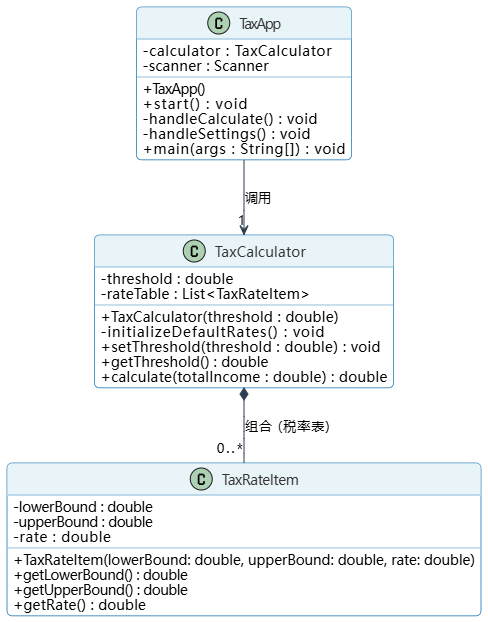
\includegraphics[width=0.75\textwidth]{img/class.png}
    \caption{核心组件 UML 类图}
    \label{fig:class}
\end{figure}

\begin{itemize}
    \item \textbf{\texttt{TaxApp} 类}：
    \begin{itemize}
        \item \textbf{私有属性（减号 \texttt{-} 表示）}：包含 \texttt{-calculator : TaxCalculator} 与 \texttt{-scanner : Scanner}，将外部依赖安全隐藏。
        \item \textbf{公有/私有方法（加号 \texttt{+} / 减号 \texttt{-} 表示）}：包含了构造函数 \texttt{+TaxApp()}、启动方法 \texttt{+start() : void}、主入口 \texttt{+main(args : String[]) : void}，以及两个被封装在内部不对外暴露的私有处理方法 \texttt{-handleCalculate() : void} 和 \texttt{-handleSettings() : void}。
        \item \textbf{依赖关系}：它通过一条标注为“\textbf{调用}”的带箭头实线指向 \texttt{TaxCalculator}，箭头旁的数字“\textbf{1}”代表一个 App 实例仅关联一个计算器引擎。
    \end{itemize}
    \item \textbf{\texttt{TaxCalculator} 类}：
    \begin{itemize}
        \item \textbf{属性与方法}：如图，不再赘述。
        \item \textbf{组合关系}：它通过一条起点为实心黑菱形的实线连接至 \texttt{TaxRateItem}。这个\textbf{实心菱形代表组合（Composition）}关系，线上的文字“组合 (税率表)”及数字“\textbf{0..*}”（代表 0 到多个）精确说明了计算器是由多条税率项构成的一个有机整体。
    \end{itemize}
    \item \textbf{\texttt{TaxRateItem} 类}：
    \begin{itemize}
        \item \textbf{属性与方法}：如图，不再赘述。
        \item 仅暴露了对应的公有（\texttt{+}）Getter 方法，确保了数据的只读安全性。
    \end{itemize}
\end{itemize}

\subsection{算法活动图}
使用活动图语法，详细刻画了 \texttt{TaxCalculator.calculate()} 方法内部的指令流转过程，如图 \ref{fig:activity} 所示。

\begin{figure}[H]
    \centering
    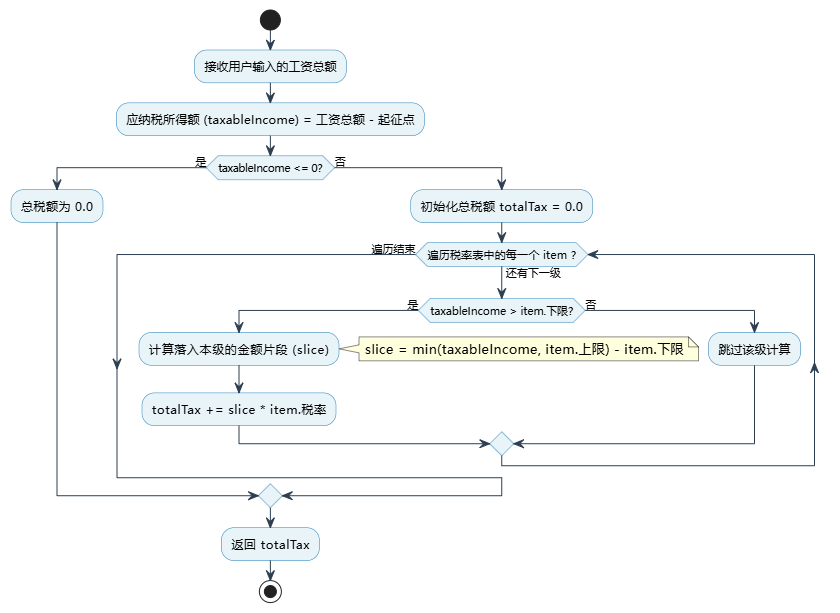
\includegraphics[width=0.75\textwidth]{img/activity.png}
    \caption{超额累进算法活动图}
    \label{fig:activity}
\end{figure}

\begin{enumerate}
    \item 首先计算应纳税所得额（总收入减去起征点）。如果结果小于等于 0，则直接返回 0 税额。
    \item 否则，进入循环遍历税率表的每一项。对于每个税率项，判断应纳税所得额是否超过该档次的下限。
    \item 如果超过，则计算该档次内的金额切片（即应纳税所得额与该档次上限的较小值减去下限），并乘以对应的税率累加到总税额中。
    \item 循环结束后返回最终计算出的总税额。
\end{enumerate}

\subsection{系统计税交互时序图}
时序图展现了系统在时间维度上的动态消息调用顺序，揭示了多个组件间是如何协同完成一次核心计税的，如图 \ref{fig:sequence} 所示。

\begin{figure}[H]
    \centering
    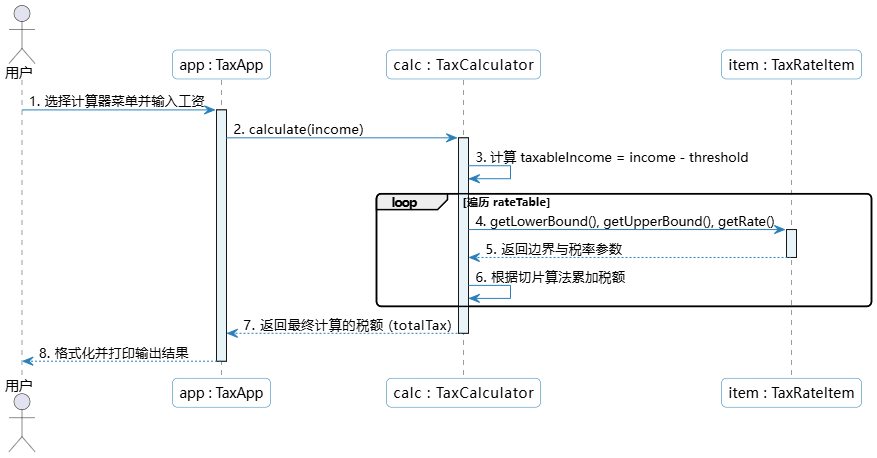
\includegraphics[width=0.75\textwidth]{img/sequence.png}
    \caption{系统计税交互时序图}
    \label{fig:sequence}
\end{figure}

如图所示，用户输入总收入后，\texttt{TaxApp} 通过调用 \texttt{TaxCalculator.calculate()} 方法，将输入数据传递给业务逻辑层。计算器内部根据税率表进行分段计算，并将结果返回给 \texttt{TaxApp}，最终由 UI 层负责输出结果给用户。

\section{算法与设计分析}

\subsection{摒弃 \texttt{if-else} 的超额累进算法}
在 \texttt{TaxCalculator} 的核心方法 \texttt{calculate} 中，摒弃了传统的阶梯式 \texttt{if-else} 或 \texttt{switch-case} 判定结构，转而采用遍历税率表对象的切片累加算法:

\begin{lstlisting}[caption={核心切片累加算法}, label={lst:calc}]
public double calculate(double totalIncome) {
    double taxableIncome = totalIncome - threshold;
    if (taxableIncome <= 0) return 0.0;

    double totalTax = 0.0;
    for (TaxRateItem item : rateTable) {
        if (taxableIncome > item.getLowerBound()) {
            // 计算落在该档次内的金额切片
            double slice = Math.min(taxableIncome, item.getUpperBound()) - item.getLowerBound();
            totalTax += slice * item.getRate();
        }
    }
    return totalTax;
}
\end{lstlisting}

\subsection{扩展性优势}
得益于上述面向对象的数据抽象与循环遍历算法，如果未来个税政策发生根本性改变（如增设超高收入人群的 6级、7级税率），\textbf{核心算法代码 (\texttt{calculate} 方法) 无需进行任何修改}。开发者仅需在系统初始化阶段，向 \texttt{rateTable} 列表中动态 \texttt{add()} 新的 \texttt{TaxRateItem} 实例即可。这深刻体现了面向对象建模在应对复杂多变业务时的扩展性。

\subsection{程序的健壮性}
在 \texttt{TaxApp} 的交互层，广泛使用了 \texttt{try-catch} 异常捕获机制。当用户在要求输入金额的环节输入非法字符（如字母或特殊符号）时，程序能够拦截 \texttt{NumberFormatException}，并友好地提示“输入数据格式不正确”，随后安全返回主菜单。这极大增强了系统的健壮性。

\subsection{自动化回归测试 (Regression Testing)}
为了验证系统的准确性并防止未来的修改引入新漏洞，系统构建了自动化回归测试模块：
\begin{enumerate}
    \item \textbf{测试用例库}：在 \texttt{test\_cases} 目录下，设计了包含普通收入用例、临界点边界值用例（如收入恰好等于起征点）、极高收入用例以及非法输入用例的结构化测试集。
    \item \textbf{批处理脚本集成}：编写了 \texttt{regression\_test.bat} 脚本。当调整了起征点逻辑或新增税率后，一键运行该脚本，即可通过 I/O 重定向将测试集的数据批量输入程序，并将结果汇总至 \texttt{test\_report.log} 中。。
\end{enumerate}


\end{document}